\documentclass{article}
\usepackage{graphicx}
\usepackage{booktabs}
\usepackage[margin=1in]{geometry}
\usepackage{float}  
\usepackage{adjustbox}  
\usepackage{amsmath}
\usepackage{cite}

\begin{document}

\title{Generated Model Performance Report}
\author{Simon Green}
\date{\today}
\maketitle

\section{Results and Model Comparison} 

This report presents the performance evaluation of four reinforcement learning models: TRPO, PPO, TRPOER, and TRPOR. These models are implemented using \textbf{Stable Baselines3} and utilize \textbf{mini-batch gradient descent} for optimization, ensuring efficient and stable updates during training. The entropy calculations guiding the models are based on the entropy of each batch, which influences regularization and experience replay mechanisms. 


\subsection{TRPO (Trust Region Policy Optimization)}

Originally proposed by Schulman et al. \cite{schulman2015trust}, TRPO is a policy gradient method that constrains updates using a trust region to ensure stability in training.

\subsection{PPO (Proximal Policy Optimization)}

Introduced by Schulman et al. \cite{schulman2017proximal}, PPO improves upon TRPO by using a clipped surrogate objective to ensure efficient and stable policy updates.

\subsection{TRPOR (TRPO with Entropy Regularization)}

This model extends TRPO by introducing entropy regularization only in the policy objective. The entropy coefficient hyperparameter guides the degree of regularization, ensuring a balance between exploration and exploitation. The entropy guiding this model is computed at the batch level, dynamically adjusting policy updates.

\subsection{TRPOER (TRPO with Entropy Regularized Experience Replay)}

This model extends TRPO by incorporating entropy-based experience replay and an additional policy entropy regularization term. It utilizes a prioritized experience replay buffer sampled according to batch entropy values and a hyperparameter coefficient. The method enables bidirectional adaptive sampling, adjusting both the number and direction of sampled experiences to optimize learning. The adaptive sampling function is formulated as:

\begin{equation}
    S = \text{clip} \left( \left( M - m \right) \times 
    \begin{cases}
        1 - \left| \frac{H}{| \lambda + \epsilon |} \right|, & \lambda > 0 \\
        \left| \frac{H}{| \lambda + \epsilon |} \right|, & \lambda < 0
    \end{cases}
    + m, \; m, \; M \right)
\end{equation}

where \( S \) is the number of samples, \( H \) represents batch entropy, \( \lambda \) is the sampling coefficient, and \( M, m \) are the maximum and minimum sample limits.


\subsection*{Model Performance Table}

The table below summarizes the models' performance in terms of mean and standard deviation of rewards, along with maximum and minimum rewards recorded during training. A higher mean reward suggests better overall performance, while lower standard deviation indicates increased stability.

\bigskip

\begin{center}
  \begin{tabular}{|l|p{3.2cm}|p{3.2cm}|p{3.2cm}|p{3.2cm}|}
\toprule
 & Ant-v5 & Pendulum-v1 & InvertedDouble Pendulum-v5 & Humanoid-v5 \\
\midrule
PPO & $\begin{array}{c} 1173.61M \\ 515.51\mu \pm 326.48\sigma \\ 1895E, 10R \end{array}$ & $\begin{array}{c} -0.02M \\ -207.56\mu \pm 118.01\sigma \\ 2892E, 10R \end{array}$ & $\begin{array}{c} 9359.93M \\ 1090.87\mu \pm 2910.66\sigma \\ 6965E, 10R \end{array}$ & $\begin{array}{c} 1245.44M \\ 464.88\mu \pm 298.07\sigma \\ 15385E, 9R \end{array}$ \\  \hline
TRPO & $\begin{array}{c} 1960.61M \\ 1328.68\mu \pm 284.88\sigma \\ 1067E, 10R \end{array}$ & $\begin{array}{c} -0.20M \\ -141.97\mu \pm 115.55\sigma \\ 2600E, 10R \end{array}$ & $\begin{array}{c} 9359.78M \\ 7516.76\mu \pm 3879.62\sigma \\ 5767E, 10R \end{array}$ & $\begin{array}{c} 1247.77M \\ 369.87\mu \pm 311.76\sigma \\ 9569E, 10R \end{array}$ \\  \hline
TRPOER & $\begin{array}{c} 1349.85M \\ 639.65\mu \pm 465.91\sigma \\ 1882E, 8R \end{array}$ & $\begin{array}{c} -0.07M \\ -173.49\mu \pm 156.48\sigma \\ 2859E, 10R \end{array}$ & $\begin{array}{c} 9351.73M \\ 2673.08\mu \pm 2620.77\sigma \\ 5070E, 9R \end{array}$ & $\begin{array}{c} 897.72M \\ 371.33\mu \pm 359.99\sigma \\ 2799E, 4R \end{array}$ \\  \hline
TRPOR & $\begin{array}{c} 3590.62M \\ 1662.87\mu \pm 1171.26\sigma \\ 1655E, 7R \end{array}$ & $\begin{array}{c} -0.22M \\ -197.32\mu \pm 215.34\sigma \\ 4508E, 10R \end{array}$ & $\begin{array}{c} 9357.32M \\ 8045.50\mu \pm 2918.29\sigma \\ 9123E, 5R \end{array}$ & $\begin{array}{c} 1416.67M \\ 620.72\mu \pm 381.70\sigma \\ 9225E, 10R \end{array}$ \\  \hline
\bottomrule  \hline
\end{tabular}

\end{center}
\
\bigskip

\section{Performance Analysis Through Plots}

The following plots visualize different aspects of model performance.

\subsection*{Learning Stability}

\begin{figure}[H]
    \centering
    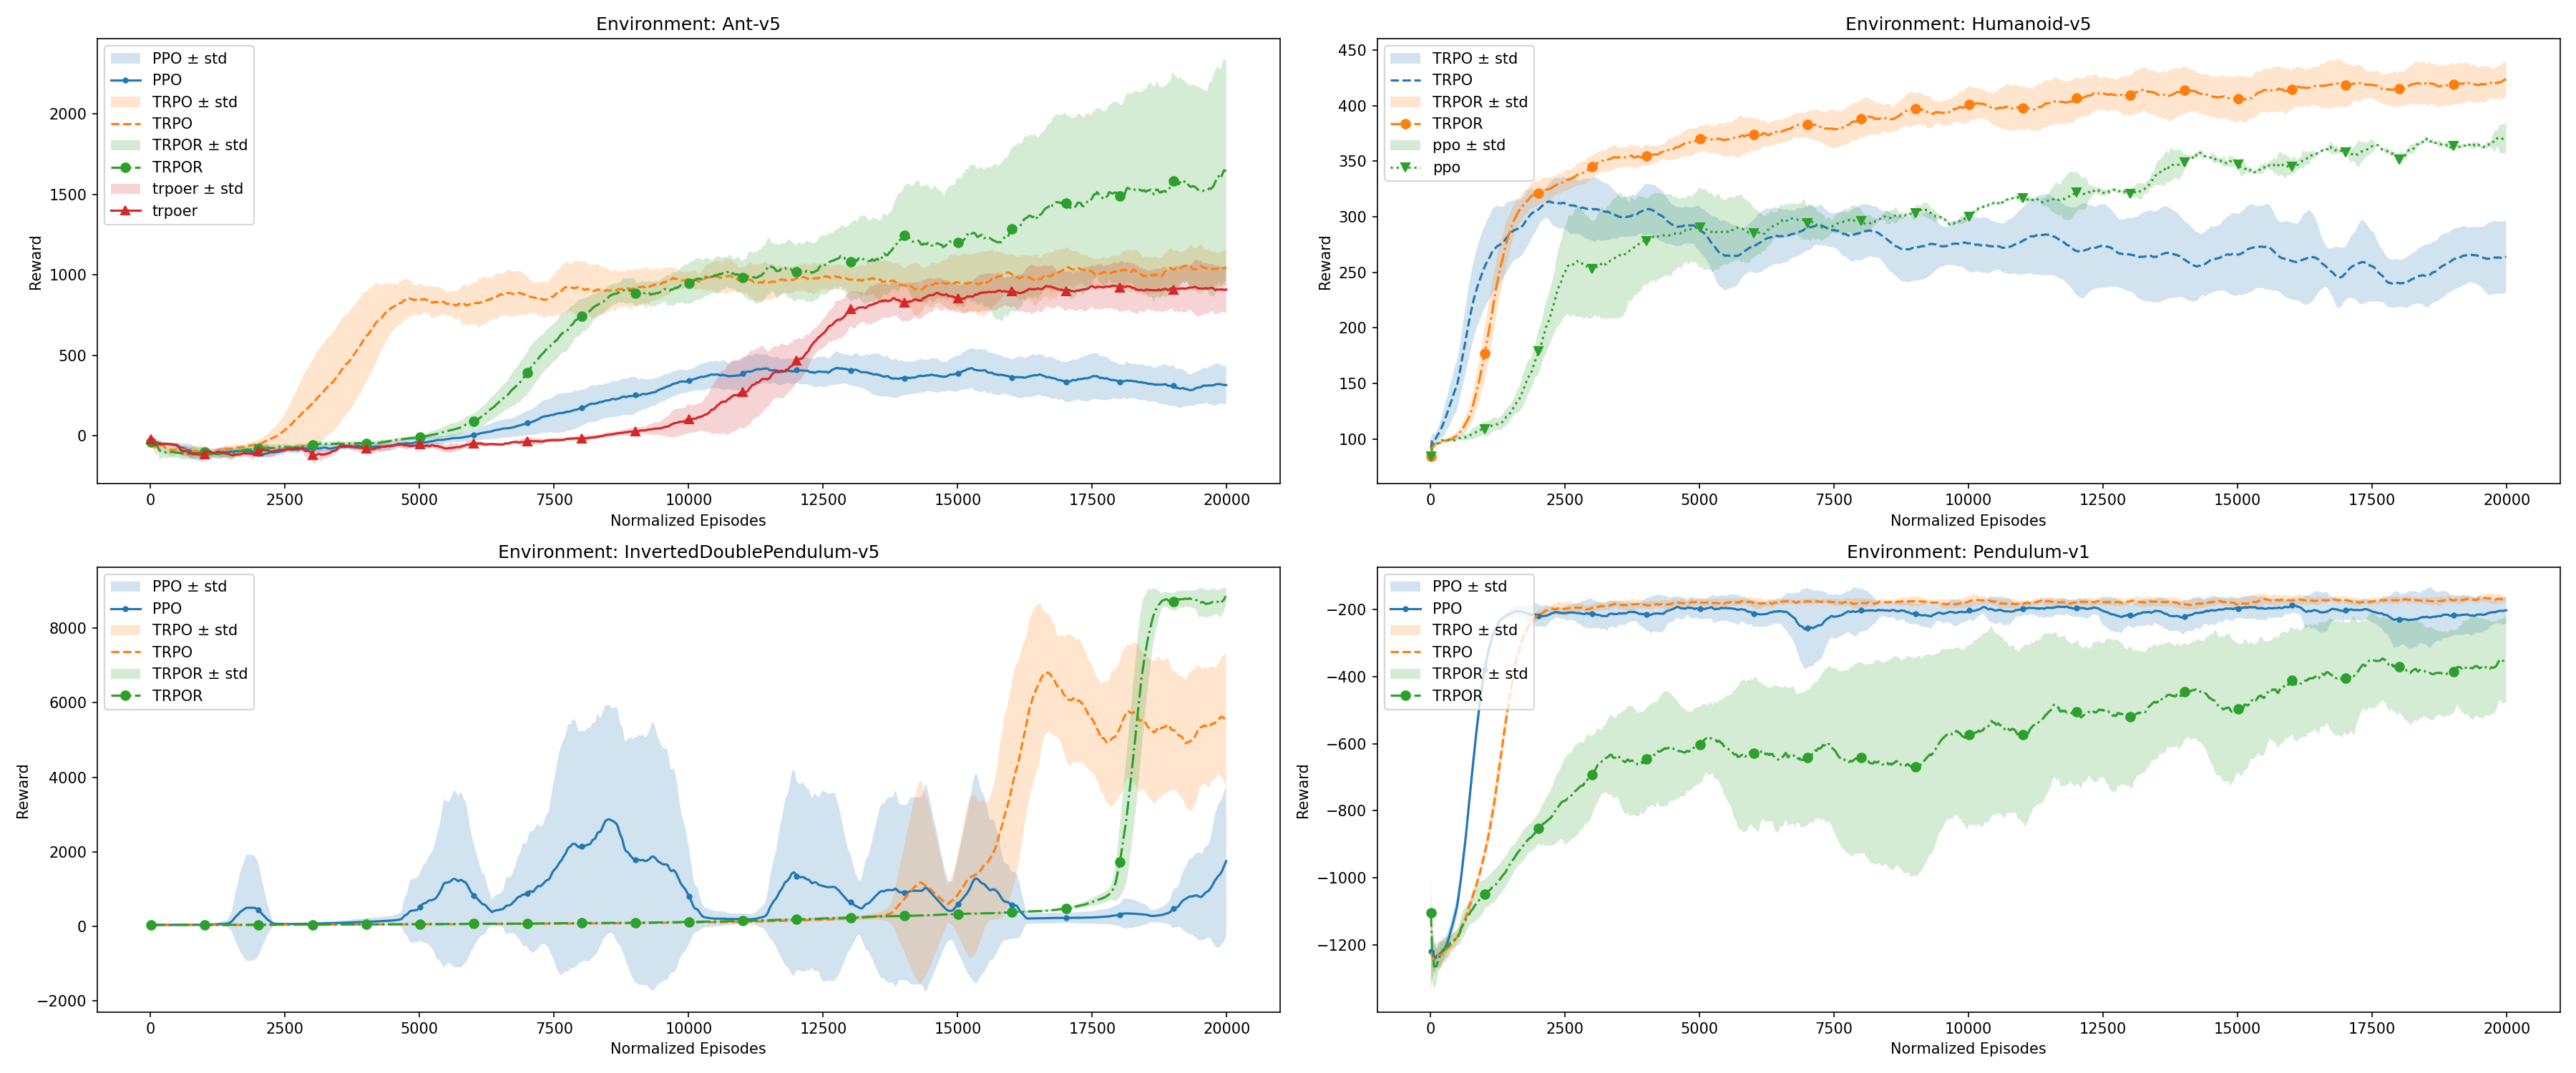
\includegraphics[width=0.8\textwidth]{.assets/learning_stability.png}
    \caption{Learning Stability for Different Models}
\end{figure}

Learning stability is evaluated based on the smoothness of the reward curve. A more stable learning process exhibits a steadily increasing reward trajectory, whereas high variance suggests instability due to sensitivity to hyperparameters.

\subsection*{Learning Stability (Coefficient of Variation)}

\begin{figure}[H]
    \centering
    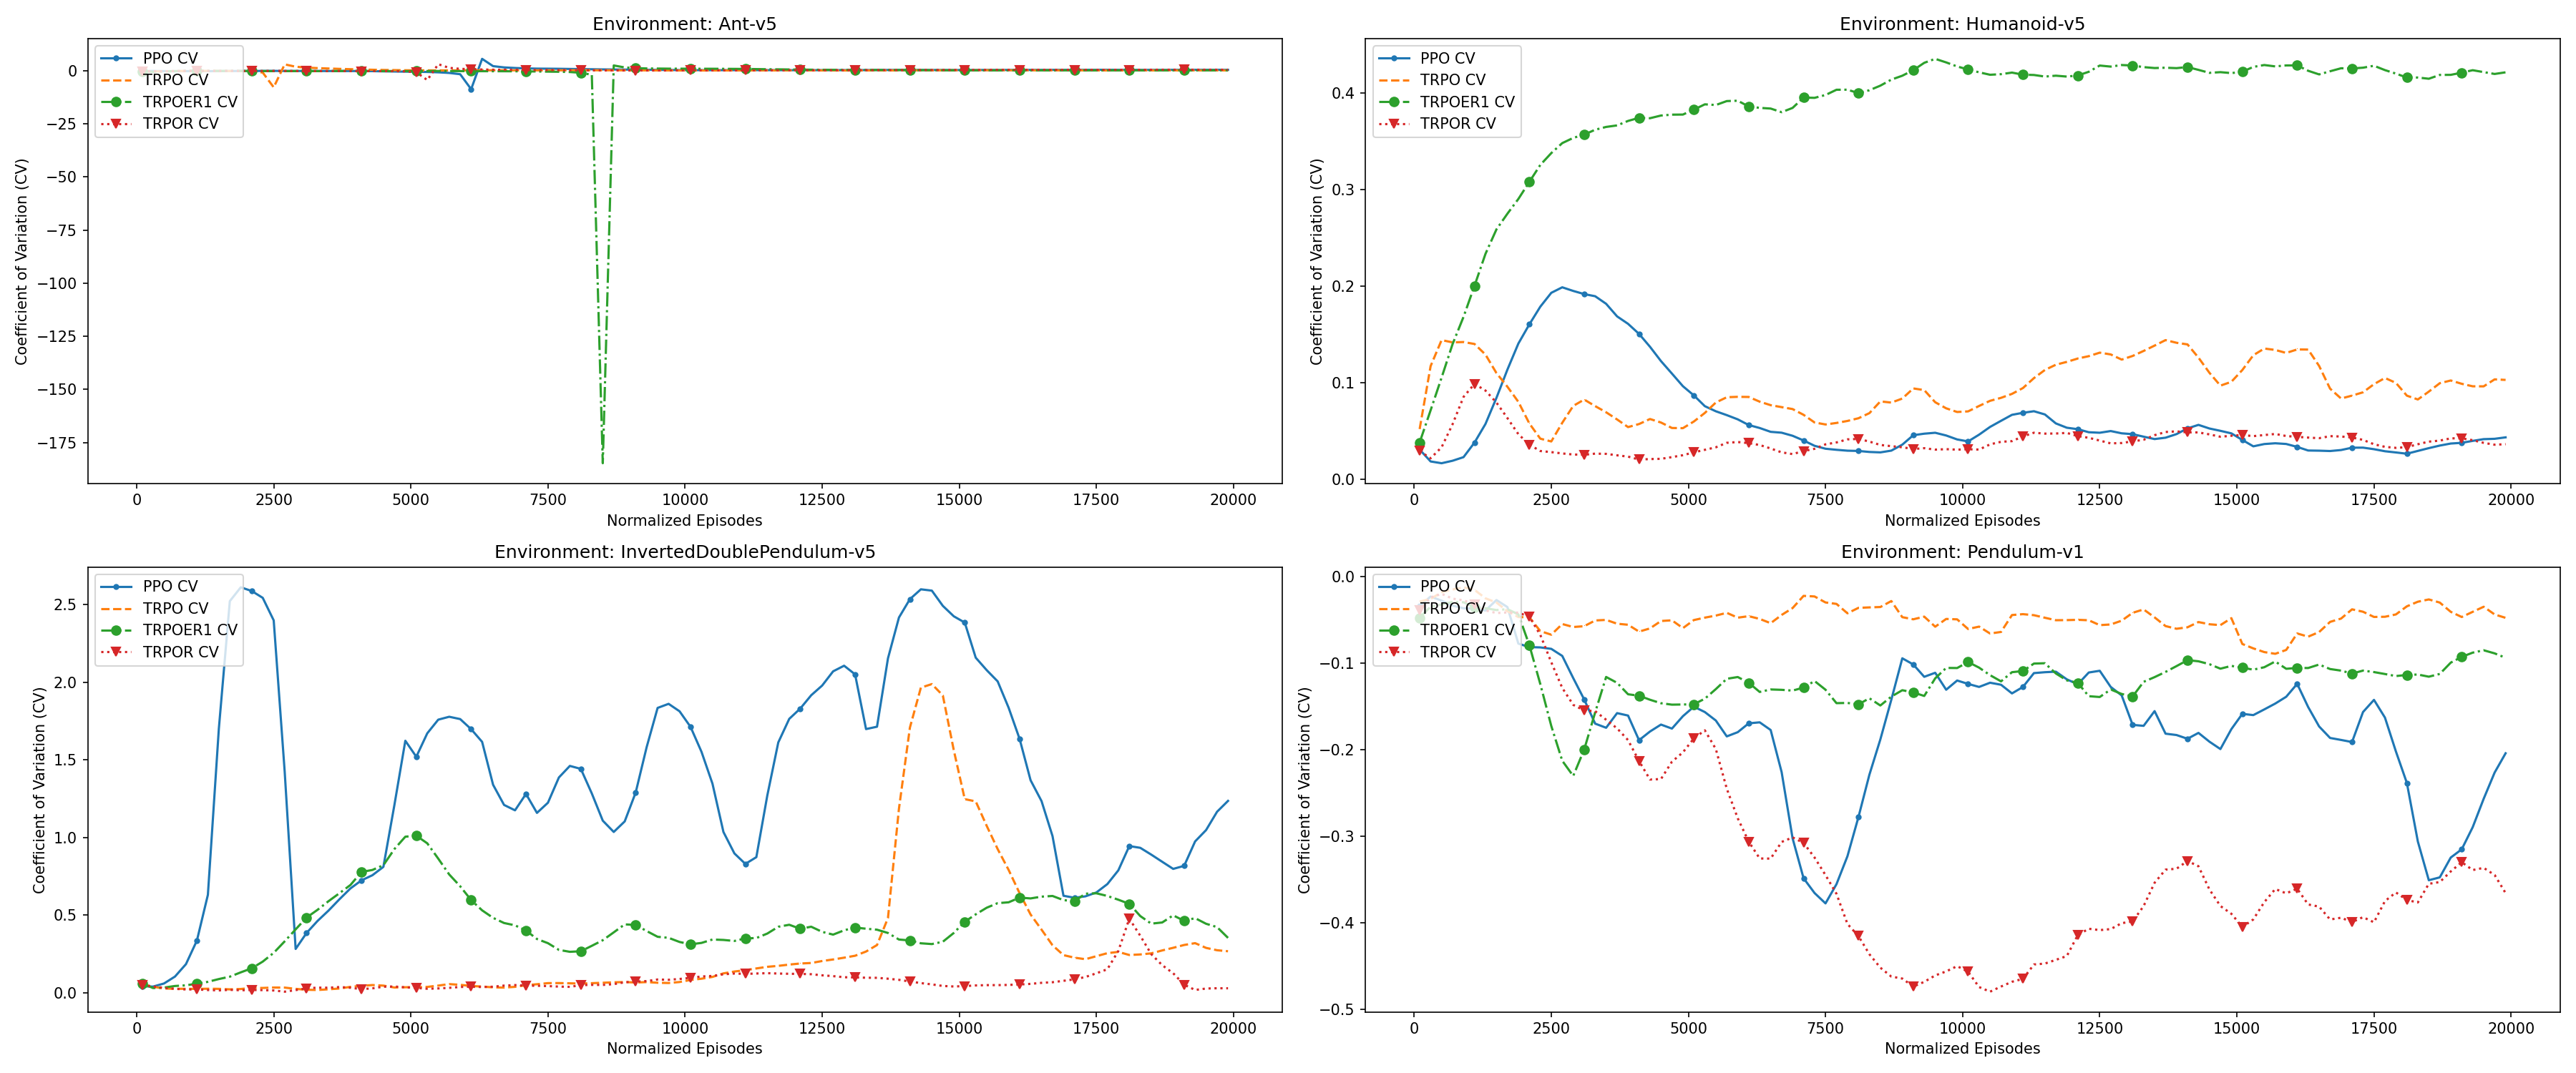
\includegraphics[width=0.8\textwidth]{.assets/learning_stability_cv.png}
    \caption{Learning Stability (Coefficient of Variation)}
\end{figure}

The coefficient of variation (CV) provides a normalized measure of stability. A lower CV signifies less volatile performance, whereas a higher CV indicates inconsistency due to randomness in training.

\subsection*{Sample Efficiency}

\begin{figure}[H]
    \centering
    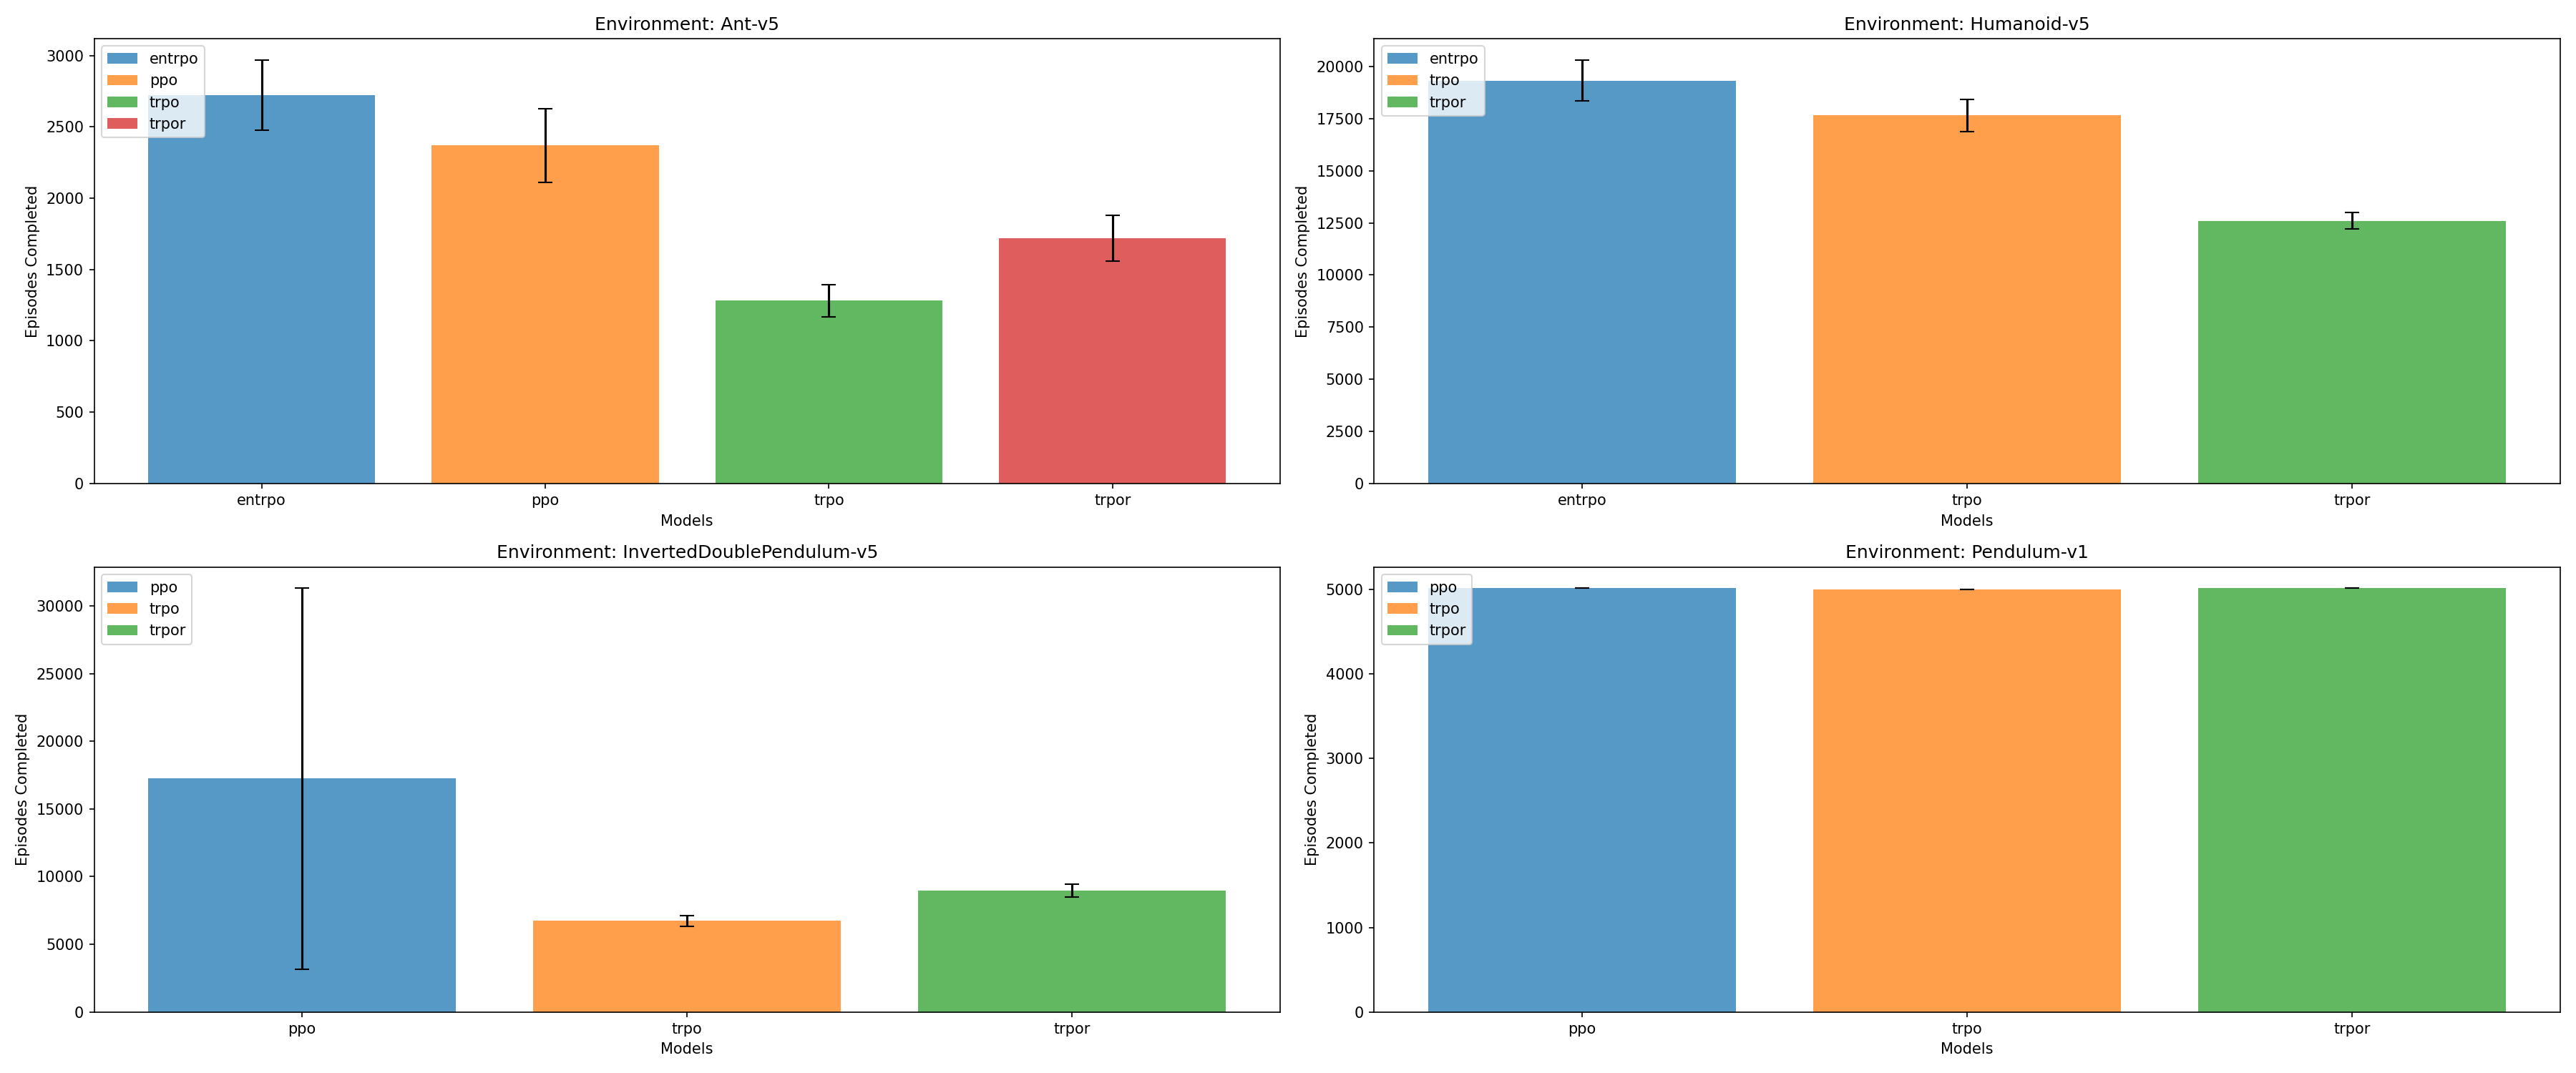
\includegraphics[width=0.8\textwidth]{.assets/sample_efficiency.png}
    \caption{Sample Efficiency Across Models}
\end{figure}

Sample efficiency measures how quickly a model improves with limited training episodes. Higher sample efficiency is desirable, especially in data-scarce scenarios.

\subsection*{Combined Sample Efficiency Results}

\begin{figure}[H]
    \centering
    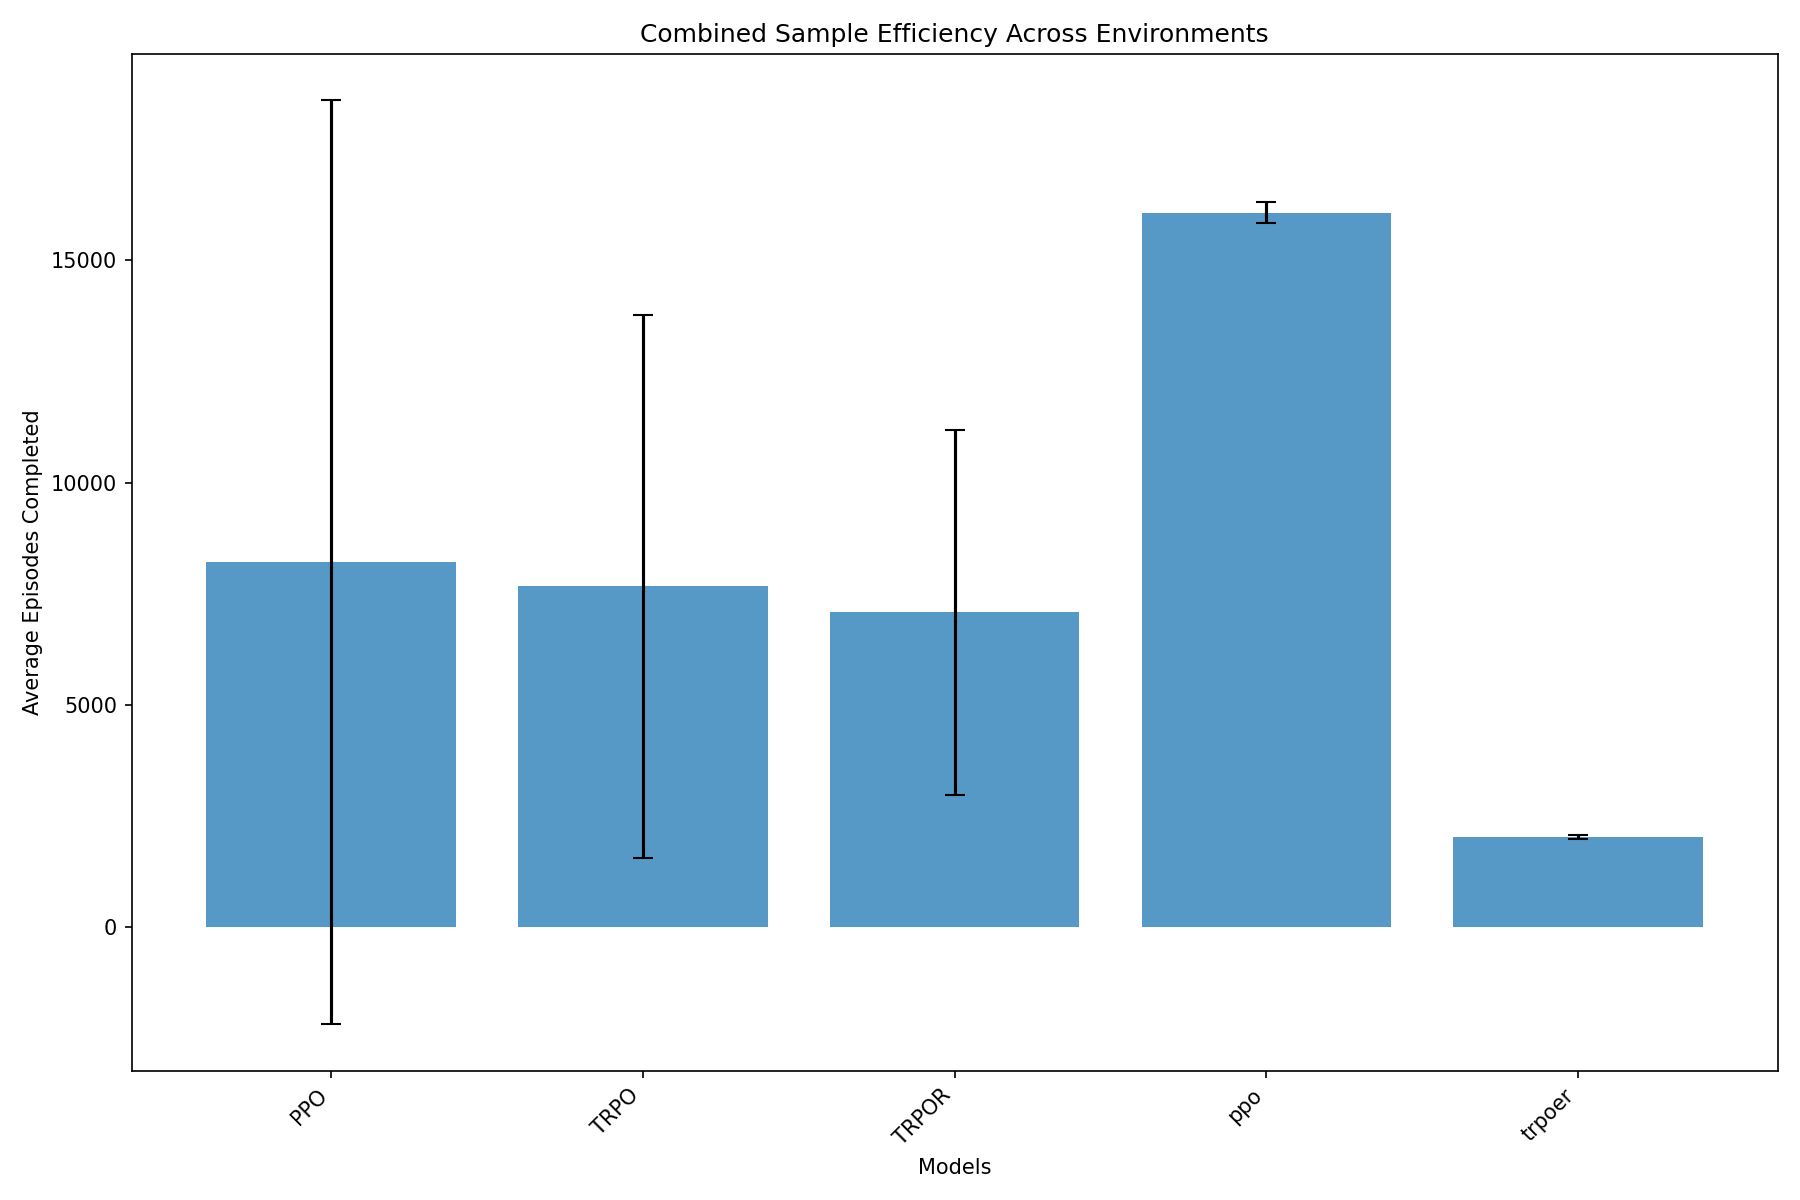
\includegraphics[width=0.8\textwidth]{.assets/sample_efficiency_combined.png}
    \caption{Combined Sample Efficiency Results}
\end{figure}

The combined sample efficiency plot aggregates results across all environments, showing how different models perform in terms of data efficiency.

\subsection*{Resampled Rewards and Outlier Removal}

\begin{figure}[H]
    \centering
    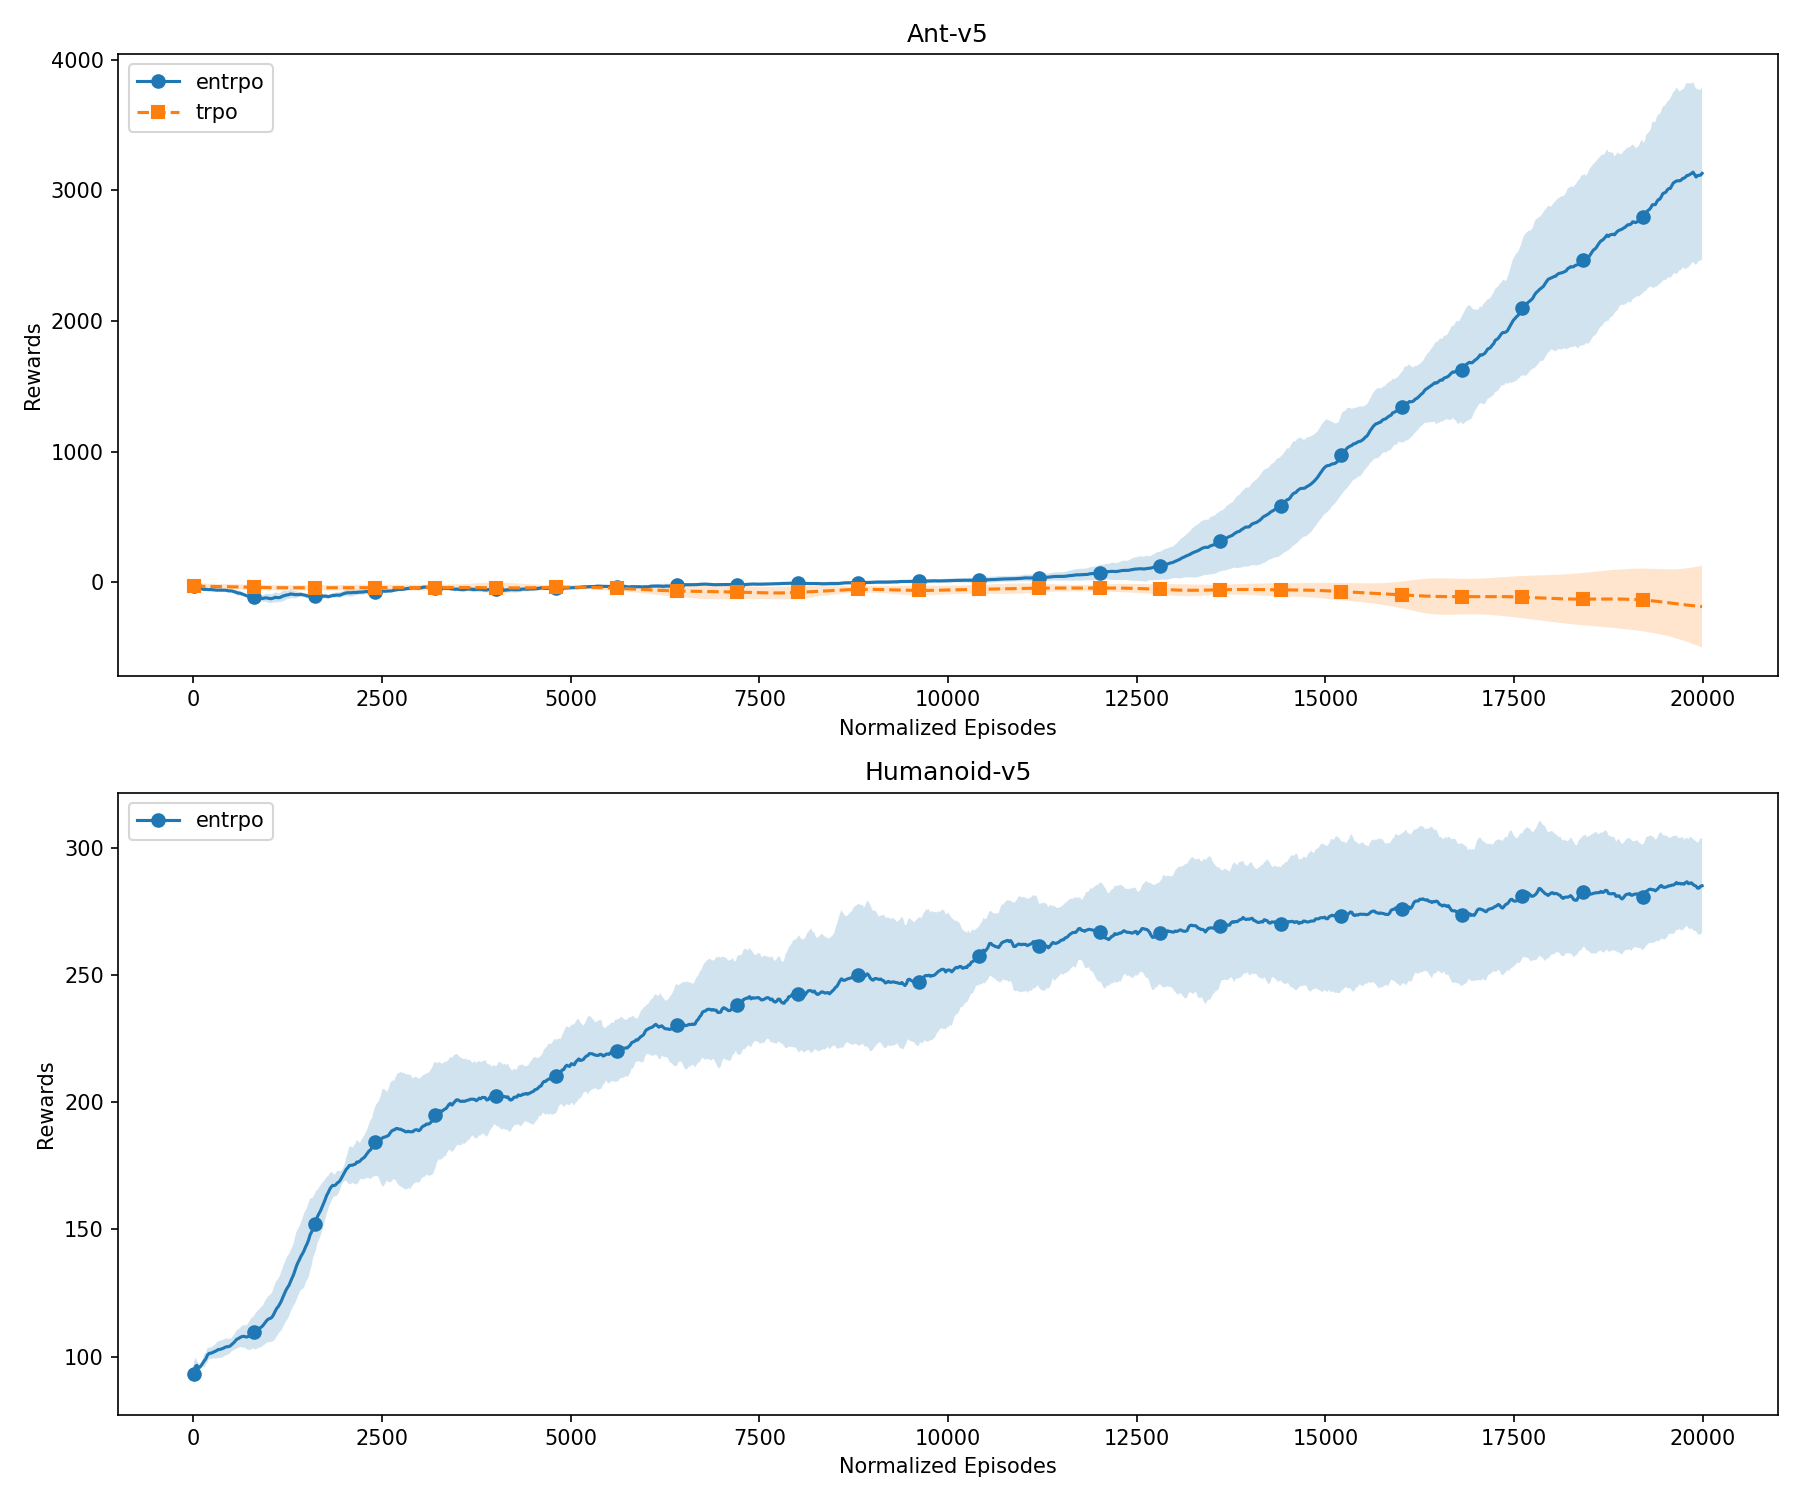
\includegraphics[width=0.8\textwidth]{.assets/resampled_outlier.png}
    \caption{Resampled Rewards with Outlier Removal}
\end{figure}

This plot presents reward distributions after applying smoothing and outlier removal techniques, filtering out misleading fluctuations.

\subsection*{Raw Data}

\begin{figure}[H]
    \centering
    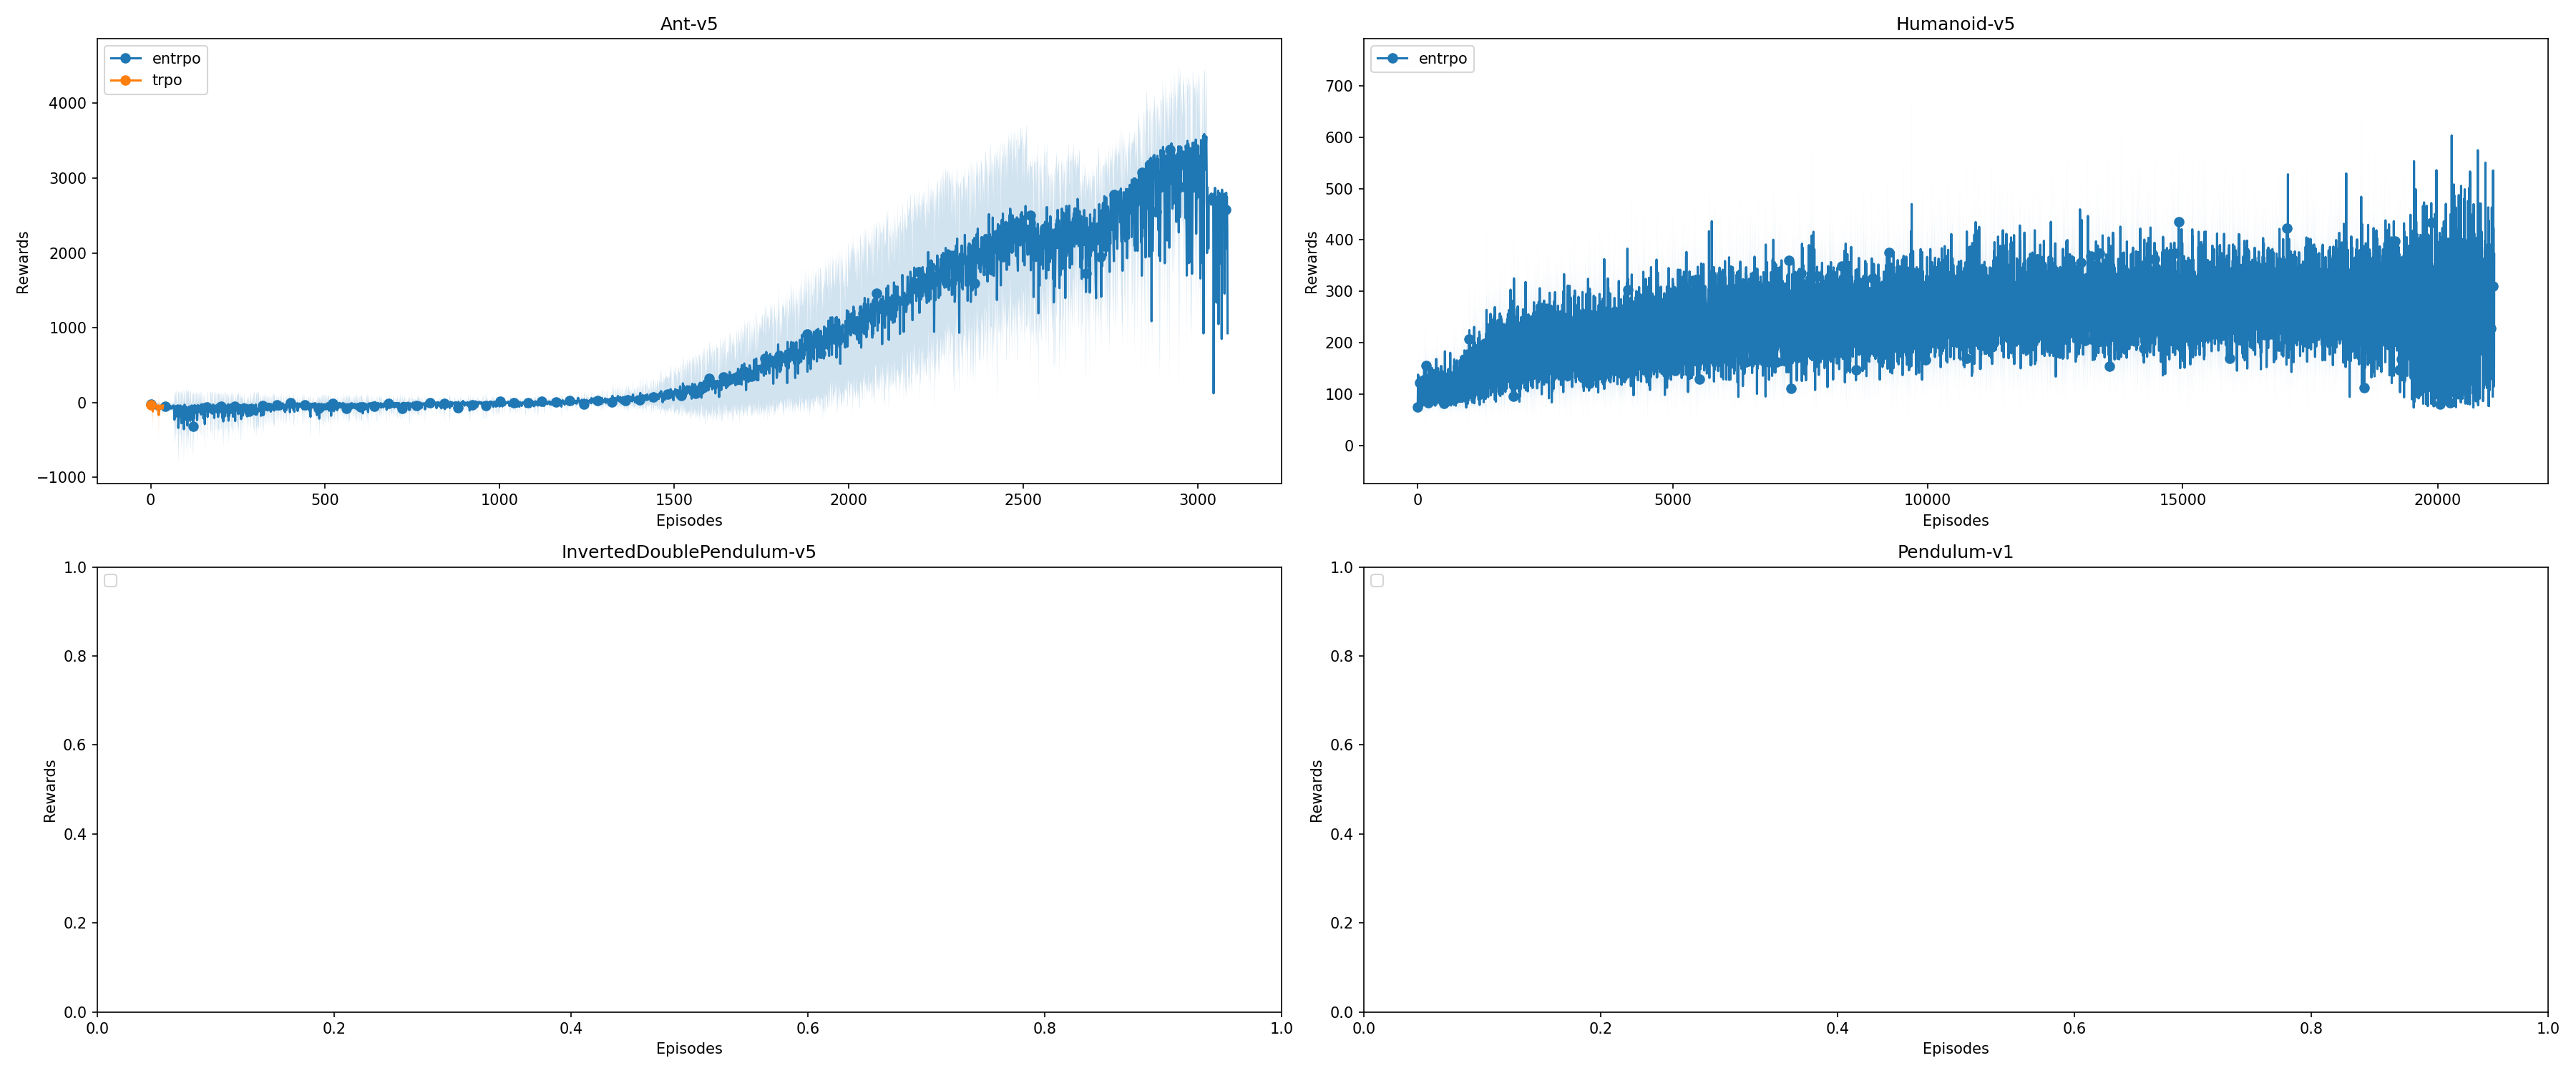
\includegraphics[width=0.8\textwidth]{.assets/raw_data.png}
    \caption{Raw Reward Data for Different Models}
\end{figure}

The raw data plot displays the recorded reward values without any smoothing. It provides insights into the actual training process and variability in rewards.

\begin{thebibliography}{9}
\bibitem{schulman2015trust} J. Schulman, S. Levine, P. Abbeel, M. Jordan, and P. Moritz, "Trust Region Policy Optimization," \textit{International Conference on Machine Learning (ICML)}, 2015.
\bibitem{schulman2017proximal} J. Schulman, F. Wolski, P. Dhariwal, A. Radford, and O. Klimov, "Proximal Policy Optimization Algorithms," \textit{arXiv preprint arXiv:1707.06347}, 2017.
\end{thebibliography}

\end{document}
